% Options for packages loaded elsewhere
\PassOptionsToPackage{unicode}{hyperref}
\PassOptionsToPackage{hyphens}{url}
%
\documentclass[
]{book}
\usepackage{lmodern}
\usepackage{amsmath}
\usepackage{ifxetex,ifluatex}
\ifnum 0\ifxetex 1\fi\ifluatex 1\fi=0 % if pdftex
  \usepackage[T1]{fontenc}
  \usepackage[utf8]{inputenc}
  \usepackage{textcomp} % provide euro and other symbols
  \usepackage{amssymb}
\else % if luatex or xetex
  \usepackage{unicode-math}
  \defaultfontfeatures{Scale=MatchLowercase}
  \defaultfontfeatures[\rmfamily]{Ligatures=TeX,Scale=1}
\fi
% Use upquote if available, for straight quotes in verbatim environments
\IfFileExists{upquote.sty}{\usepackage{upquote}}{}
\IfFileExists{microtype.sty}{% use microtype if available
  \usepackage[]{microtype}
  \UseMicrotypeSet[protrusion]{basicmath} % disable protrusion for tt fonts
}{}
\makeatletter
\@ifundefined{KOMAClassName}{% if non-KOMA class
  \IfFileExists{parskip.sty}{%
    \usepackage{parskip}
  }{% else
    \setlength{\parindent}{0pt}
    \setlength{\parskip}{6pt plus 2pt minus 1pt}}
}{% if KOMA class
  \KOMAoptions{parskip=half}}
\makeatother
\usepackage{xcolor}
\IfFileExists{xurl.sty}{\usepackage{xurl}}{} % add URL line breaks if available
\IfFileExists{bookmark.sty}{\usepackage{bookmark}}{\usepackage{hyperref}}
\hypersetup{
  pdftitle={2수준 요인법 - 교락법 실습},
  pdfauthor={서울시립대 통계학과},
  hidelinks,
  pdfcreator={LaTeX via pandoc}}
\urlstyle{same} % disable monospaced font for URLs
\usepackage{color}
\usepackage{fancyvrb}
\newcommand{\VerbBar}{|}
\newcommand{\VERB}{\Verb[commandchars=\\\{\}]}
\DefineVerbatimEnvironment{Highlighting}{Verbatim}{commandchars=\\\{\}}
% Add ',fontsize=\small' for more characters per line
\usepackage{framed}
\definecolor{shadecolor}{RGB}{248,248,248}
\newenvironment{Shaded}{\begin{snugshade}}{\end{snugshade}}
\newcommand{\AlertTok}[1]{\textcolor[rgb]{0.94,0.16,0.16}{#1}}
\newcommand{\AnnotationTok}[1]{\textcolor[rgb]{0.56,0.35,0.01}{\textbf{\textit{#1}}}}
\newcommand{\AttributeTok}[1]{\textcolor[rgb]{0.77,0.63,0.00}{#1}}
\newcommand{\BaseNTok}[1]{\textcolor[rgb]{0.00,0.00,0.81}{#1}}
\newcommand{\BuiltInTok}[1]{#1}
\newcommand{\CharTok}[1]{\textcolor[rgb]{0.31,0.60,0.02}{#1}}
\newcommand{\CommentTok}[1]{\textcolor[rgb]{0.56,0.35,0.01}{\textit{#1}}}
\newcommand{\CommentVarTok}[1]{\textcolor[rgb]{0.56,0.35,0.01}{\textbf{\textit{#1}}}}
\newcommand{\ConstantTok}[1]{\textcolor[rgb]{0.00,0.00,0.00}{#1}}
\newcommand{\ControlFlowTok}[1]{\textcolor[rgb]{0.13,0.29,0.53}{\textbf{#1}}}
\newcommand{\DataTypeTok}[1]{\textcolor[rgb]{0.13,0.29,0.53}{#1}}
\newcommand{\DecValTok}[1]{\textcolor[rgb]{0.00,0.00,0.81}{#1}}
\newcommand{\DocumentationTok}[1]{\textcolor[rgb]{0.56,0.35,0.01}{\textbf{\textit{#1}}}}
\newcommand{\ErrorTok}[1]{\textcolor[rgb]{0.64,0.00,0.00}{\textbf{#1}}}
\newcommand{\ExtensionTok}[1]{#1}
\newcommand{\FloatTok}[1]{\textcolor[rgb]{0.00,0.00,0.81}{#1}}
\newcommand{\FunctionTok}[1]{\textcolor[rgb]{0.00,0.00,0.00}{#1}}
\newcommand{\ImportTok}[1]{#1}
\newcommand{\InformationTok}[1]{\textcolor[rgb]{0.56,0.35,0.01}{\textbf{\textit{#1}}}}
\newcommand{\KeywordTok}[1]{\textcolor[rgb]{0.13,0.29,0.53}{\textbf{#1}}}
\newcommand{\NormalTok}[1]{#1}
\newcommand{\OperatorTok}[1]{\textcolor[rgb]{0.81,0.36,0.00}{\textbf{#1}}}
\newcommand{\OtherTok}[1]{\textcolor[rgb]{0.56,0.35,0.01}{#1}}
\newcommand{\PreprocessorTok}[1]{\textcolor[rgb]{0.56,0.35,0.01}{\textit{#1}}}
\newcommand{\RegionMarkerTok}[1]{#1}
\newcommand{\SpecialCharTok}[1]{\textcolor[rgb]{0.00,0.00,0.00}{#1}}
\newcommand{\SpecialStringTok}[1]{\textcolor[rgb]{0.31,0.60,0.02}{#1}}
\newcommand{\StringTok}[1]{\textcolor[rgb]{0.31,0.60,0.02}{#1}}
\newcommand{\VariableTok}[1]{\textcolor[rgb]{0.00,0.00,0.00}{#1}}
\newcommand{\VerbatimStringTok}[1]{\textcolor[rgb]{0.31,0.60,0.02}{#1}}
\newcommand{\WarningTok}[1]{\textcolor[rgb]{0.56,0.35,0.01}{\textbf{\textit{#1}}}}
\usepackage{longtable,booktabs}
\usepackage{calc} % for calculating minipage widths
% Correct order of tables after \paragraph or \subparagraph
\usepackage{etoolbox}
\makeatletter
\patchcmd\longtable{\par}{\if@noskipsec\mbox{}\fi\par}{}{}
\makeatother
% Allow footnotes in longtable head/foot
\IfFileExists{footnotehyper.sty}{\usepackage{footnotehyper}}{\usepackage{footnote}}
\makesavenoteenv{longtable}
\usepackage{graphicx}
\makeatletter
\def\maxwidth{\ifdim\Gin@nat@width>\linewidth\linewidth\else\Gin@nat@width\fi}
\def\maxheight{\ifdim\Gin@nat@height>\textheight\textheight\else\Gin@nat@height\fi}
\makeatother
% Scale images if necessary, so that they will not overflow the page
% margins by default, and it is still possible to overwrite the defaults
% using explicit options in \includegraphics[width, height, ...]{}
\setkeys{Gin}{width=\maxwidth,height=\maxheight,keepaspectratio}
% Set default figure placement to htbp
\makeatletter
\def\fps@figure{htbp}
\makeatother
\setlength{\emergencystretch}{3em} % prevent overfull lines
\providecommand{\tightlist}{%
  \setlength{\itemsep}{0pt}\setlength{\parskip}{0pt}}
\setcounter{secnumdepth}{5}
\usepackage[onehalfspacing]{setspace}

\usepackage[hangul]{kotex}
\usepackage{fullpage}
\newcommand{\pardiff}[2]{\frac{\partial #1}{\partial #2 }}
\newcommand{\pardiffl}[2]{{\partial #1}/{\partial #2 }}
\newcommand{\pardiffd}[2]{\frac{\partial^2 #1}{\partial #2^t \partial #2 }}
\newcommand{\pardiffdd}[3]{\frac{\partial^2 #1}{\partial #2 \partial #3 }}

\newcommand{\bm}[1]{\boldsymbol{\mathbf{#1}}}

\usepackage{booktabs}
\usepackage{longtable}
\usepackage[bf,singlelinecheck=off]{caption}

%\setmainfont[UprightFeatures={SmallCapsFont=AlegreyaSC-Regular}]{Alegreya}

\usepackage{framed,color}
\definecolor{shadecolor}{RGB}{248,248,248}

\renewcommand{\textfraction}{0.05}
\renewcommand{\topfraction}{0.8}
\renewcommand{\bottomfraction}{0.8}
\renewcommand{\floatpagefraction}{0.75}

\renewenvironment{quote}{\begin{VF}}{\end{VF}}
\let\oldhref\href
\renewcommand{\href}[2]{#2\footnote{\url{#1}}}

\makeatletter
\newenvironment{kframe}{%
\medskip{}
\setlength{\fboxsep}{.8em}
 \def\at@end@of@kframe{}%
 \ifinner\ifhmode%
  \def\at@end@of@kframe{\end{minipage}}%
  \begin{minipage}{\columnwidth}%
 \fi\fi%
 \def\FrameCommand##1{\hskip\@totalleftmargin \hskip-\fboxsep
 \colorbox{shadecolor}{##1}\hskip-\fboxsep
     % There is no \\@totalrightmargin, so:
     \hskip-\linewidth \hskip-\@totalleftmargin \hskip\columnwidth}%
 \MakeFramed {\advance\hsize-\width
   \@totalleftmargin\z@ \linewidth\hsize
   \@setminipage}}%
 {\par\unskip\endMakeFramed%
 \at@end@of@kframe}
\makeatother

\makeatletter

\@ifundefined{Shaded}{
}{\renewenvironment{Shaded}{\begin{kframe}}{\end{kframe}}}
\makeatother

\newenvironment{rmdblock}[1]
  {
  \begin{itemize}
  \renewcommand{\labelitemi}{
    \raisebox{-.7\height}[0pt][0pt]{
      {\setkeys{Gin}{width=3em,keepaspectratio}\includegraphics{images/#1}}
    }
  }
  \setlength{\fboxsep}{1em}
  \begin{kframe}
  \item
  }
  {
  \end{kframe}
  \end{itemize}
  }
  
\newenvironment{rmdnote}
  {\begin{rmdblock}{note}}
  {\end{rmdblock}}
  
\newenvironment{rmdcaution}
  {\begin{rmdblock}{caution}}
  {\end{rmdblock}}
  
\newenvironment{rmdimportant}
  {\begin{rmdblock}{important}}
  {\end{rmdblock}}
  
\newenvironment{rmdtip}
  {\begin{rmdblock}{tip}}
  {\end{rmdblock}}
  
\newenvironment{rmdwarning}
  {\begin{rmdblock}{warning}}
  {\end{rmdblock}}
  


%\usepackage{makeidx}
%\makeindex

\urlstyle{tt}

\usepackage{amsthm}
\makeatletter
 \def\thm@space@setup{%
   \thm@preskip=8pt plus 2pt minus 4pt
   \thm@postskip=\thm@preskip
}
\makeatother

\frontmatter

\usepackage{booktabs}
\usepackage{longtable}
\usepackage{array}
\usepackage{multirow}
\usepackage{wrapfig}
\usepackage{float}
\usepackage{colortbl}
\usepackage{pdflscape}
\usepackage{tabu}
\usepackage{threeparttable}
\usepackage{threeparttablex}
\usepackage[normalem]{ulem}
\usepackage{makecell}
\usepackage{xcolor}
\ifluatex
  \usepackage{selnolig}  % disable illegal ligatures
\fi
\usepackage[]{natbib}
\bibliographystyle{apalike}

\title{2수준 요인법 - 교락법 실습}
\author{서울시립대 통계학과}
\date{2021-05-20}

\begin{document}
\maketitle

{
\setcounter{tocdepth}{1}
\tableofcontents
}
\hypertarget{uxc11cuxbb38}{%
\chapter*{서문}\label{uxc11cuxbb38}}


교과서 8장 2수준 요인법의 교락법에 대한 예제 풀이 강의입니다.

\begin{center}\rule{0.5\linewidth}{0.5pt}\end{center}

이 노트에 있는 R 프로그램을 실행하려면 다음과 같은 패키지들이 필요하다.

\begin{verbatim}
library(dplyr)
library(tidyr)
library(ggplot2)
library(agricolae)
library(emmeans)
library(SixSigma)
library(FrF2)
library(unrepx)
library(conf.design)
library(knitr)
library(kableExtra)
\end{verbatim}

\mainmatter

\hypertarget{ex82}{%
\chapter{교과서 예제 8.2}\label{ex82}}

반복이 없는 \(2^4\) 요인배치법에서 16회의 실험을 동일한 환경에서 실시할 수 없어서 상호작용효과 \(ACD\) 와 \(BCD\) 를 블럭과 교락시켜서 실험하였다 (교과서 예제 8.2, 230 페이지)

\hypertarget{uxc2e4uxd5d8uxc790uxb8ccuxc758-uxc0dduxc131}{%
\section{실험자료의 생성}\label{uxc2e4uxd5d8uxc790uxb8ccuxc758-uxc0dduxc131}}

먼저 16개의 실험 처리 조합을 표준 순서로서 생성하자. \texttt{default.level=c(0,1)} 은 요인의 수준을
0과 1로 표시하는 옵션이다.

\begin{Shaded}
\begin{Highlighting}[]
\NormalTok{X }\OtherTok{\textless{}{-}} \FunctionTok{FrF2}\NormalTok{(}\AttributeTok{nruns=}\DecValTok{16}\NormalTok{, }\AttributeTok{nfactors=}\DecValTok{4}\NormalTok{, }\AttributeTok{randomize =} \ConstantTok{FALSE}\NormalTok{,  }\AttributeTok{default.level=}\FunctionTok{c}\NormalTok{(}\DecValTok{0}\NormalTok{,}\DecValTok{1}\NormalTok{))}
\end{Highlighting}
\end{Shaded}

\begin{verbatim}
## creating full factorial with 16 runs ...
\end{verbatim}

\begin{Shaded}
\begin{Highlighting}[]
\NormalTok{X}
\end{Highlighting}
\end{Shaded}

\begin{verbatim}
##    A B C D
## 1  0 0 0 0
## 2  1 0 0 0
## 3  0 1 0 0
## 4  1 1 0 0
## 5  0 0 1 0
## 6  1 0 1 0
## 7  0 1 1 0
## 8  1 1 1 0
## 9  0 0 0 1
## 10 1 0 0 1
## 11 0 1 0 1
## 12 1 1 0 1
## 13 0 0 1 1
## 14 1 0 1 1
## 15 0 1 1 1
## 16 1 1 1 1
## class=design, type= full factorial
\end{verbatim}

실험의 표준 순서는 다음과 같이 \texttt{yates()} 함수를 이용하여 알 수 있다.

\begin{Shaded}
\begin{Highlighting}[]
\FunctionTok{yates}\NormalTok{(}\FunctionTok{rep}\NormalTok{(}\DecValTok{0}\NormalTok{,}\DecValTok{16}\NormalTok{))}
\end{Highlighting}
\end{Shaded}

\begin{verbatim}
##    A    B   AB    C   AC   BC  ABC    D   AD   BD  ABD   CD  ACD  BCD ABCD 
##    0    0    0    0    0    0    0    0    0    0    0    0    0    0    0 
## attr(,"mean")
##   
## 0
\end{verbatim}

그리고 처리의 표준 순서로 실험값과 블럭변수를 입력한다. 그리고 처리조합 정보 \texttt{X} 와 결합하여 최종 자료인 \texttt{df} 를 만들자.

\begin{figure}

{\centering \includegraphics[width=0.8\linewidth]{images/ex82} 

}

\caption{예제 8.2 자료}\label{fig:unnamed-chunk-4}
\end{figure}

\begin{Shaded}
\begin{Highlighting}[]
\NormalTok{y }\OtherTok{\textless{}{-}} \FunctionTok{c}\NormalTok{(}\DecValTok{45}\NormalTok{,}\DecValTok{71}\NormalTok{, }\DecValTok{48}\NormalTok{, }\DecValTok{65}\NormalTok{, }\DecValTok{68}\NormalTok{, }\DecValTok{60}\NormalTok{, }\DecValTok{80}\NormalTok{, }\DecValTok{65}\NormalTok{, }\DecValTok{43}\NormalTok{, }\DecValTok{100}\NormalTok{, }\DecValTok{45}\NormalTok{, }\DecValTok{104}\NormalTok{, }\DecValTok{75}\NormalTok{, }\DecValTok{86}\NormalTok{, }\DecValTok{70}\NormalTok{, }\DecValTok{96}\NormalTok{ )}
\NormalTok{block }\OtherTok{\textless{}{-}} \FunctionTok{factor}\NormalTok{(}\FunctionTok{c}\NormalTok{(}\DecValTok{1}\NormalTok{, }\DecValTok{3}\NormalTok{, }\DecValTok{2}\NormalTok{, }\DecValTok{4}\NormalTok{, }\DecValTok{4}\NormalTok{, }\DecValTok{2}\NormalTok{, }\DecValTok{3}\NormalTok{, }\DecValTok{1}\NormalTok{, }\DecValTok{4}\NormalTok{, }\DecValTok{2}\NormalTok{, }\DecValTok{3}\NormalTok{, }\DecValTok{1}\NormalTok{, }\DecValTok{1}\NormalTok{, }\DecValTok{3}\NormalTok{, }\DecValTok{2}\NormalTok{, }\DecValTok{4}\NormalTok{))}
\NormalTok{treat }\OtherTok{\textless{}{-}} \FunctionTok{c}\NormalTok{(}\StringTok{"0"}\NormalTok{, }\FunctionTok{names}\NormalTok{(}\FunctionTok{yates}\NormalTok{(}\FunctionTok{rep}\NormalTok{(}\DecValTok{0}\NormalTok{,}\DecValTok{16}\NormalTok{))))}
\NormalTok{df0 }\OtherTok{\textless{}{-}} \FunctionTok{data.frame}\NormalTok{(}\AttributeTok{block=}\NormalTok{block, }\AttributeTok{treat=}\NormalTok{treat,  }\AttributeTok{y=}\NormalTok{y )}
\NormalTok{df }\OtherTok{\textless{}{-}} \FunctionTok{cbind}\NormalTok{(X, df0)}
\end{Highlighting}
\end{Shaded}

\begin{Shaded}
\begin{Highlighting}[]
\NormalTok{df }\SpecialCharTok{\%\textgreater{}\%}  \FunctionTok{kbl}\NormalTok{() }\SpecialCharTok{\%\textgreater{}\%}   \FunctionTok{kable\_paper}\NormalTok{(}\StringTok{"hover"}\NormalTok{, }\AttributeTok{full\_width =}\NormalTok{ F)}
\end{Highlighting}
\end{Shaded}

\begin{table}
\centering
\begin{tabular}[t]{l|l|l|l|l|l|r}
\hline
A & B & C & D & block & treat & y\\
\hline
0 & 0 & 0 & 0 & 1 & 0 & 45\\
\hline
1 & 0 & 0 & 0 & 3 & A & 71\\
\hline
0 & 1 & 0 & 0 & 2 & B & 48\\
\hline
1 & 1 & 0 & 0 & 4 & AB & 65\\
\hline
0 & 0 & 1 & 0 & 4 & C & 68\\
\hline
1 & 0 & 1 & 0 & 2 & AC & 60\\
\hline
0 & 1 & 1 & 0 & 3 & BC & 80\\
\hline
1 & 1 & 1 & 0 & 1 & ABC & 65\\
\hline
0 & 0 & 0 & 1 & 4 & D & 43\\
\hline
1 & 0 & 0 & 1 & 2 & AD & 100\\
\hline
0 & 1 & 0 & 1 & 3 & BD & 45\\
\hline
1 & 1 & 0 & 1 & 1 & ABD & 104\\
\hline
0 & 0 & 1 & 1 & 1 & CD & 75\\
\hline
1 & 0 & 1 & 1 & 3 & ACD & 86\\
\hline
0 & 1 & 1 & 1 & 2 & BCD & 70\\
\hline
1 & 1 & 1 & 1 & 4 & ABCD & 96\\
\hline
\end{tabular}
\end{table}

위의 실험 자료를 블럭과 처리 순으로 정렬해 보자.

\begin{Shaded}
\begin{Highlighting}[]
\NormalTok{df }\SpecialCharTok{\%\textgreater{}\%} \FunctionTok{arrange}\NormalTok{( block, treat)}
\end{Highlighting}
\end{Shaded}

\begin{verbatim}
##    A B C D block treat   y
## 1  0 0 0 0     1     0  45
## 2  1 1 1 0     1   ABC  65
## 3  1 1 0 1     1   ABD 104
## 4  0 0 1 1     1    CD  75
## 5  1 0 1 0     2    AC  60
## 6  1 0 0 1     2    AD 100
## 7  0 1 0 0     2     B  48
## 8  0 1 1 1     2   BCD  70
## 9  1 0 0 0     3     A  71
## 10 1 0 1 1     3   ACD  86
## 11 0 1 1 0     3    BC  80
## 12 0 1 0 1     3    BD  45
## 13 1 1 0 0     4    AB  65
## 14 1 1 1 1     4  ABCD  96
## 15 0 0 1 0     4     C  68
## 16 0 0 0 1     4     D  43
\end{verbatim}

\hypertarget{uxc120uxd615uxd45cuxd604uxc2dd}{%
\section{선형표현식}\label{uxc120uxd615uxd45cuxd604uxc2dd}}

이제 위에서 생성된 자료에서 상호작용효과 \(ACD\) 와 \(BCD\) 가 블록과 교락되어 있는지
선형표현식을 이용하여 확인해 보자.

\begin{align*}
L_1 & = x_1 + x_3 + x_4 (\text{mod}2) \\
L_2 & = x_2 + x_3 + x_4 (\text{mod}2)
\end{align*}

예를 들어 블럭 1 (\(L_1=0, L_2=0\)) 에 베치된 처리에 대하여 선형식의 값을 구해보자.

\begin{longtable}[]{@{}cccc@{}}
\toprule
블럭 & 처리 & \(L_1 (ACD)\) & \(L_2 (BCD)\)\tabularnewline
\midrule
\endhead
1 & \((0)\) & \(\texttt{MOD} (0+0+0, 2) = 0\) & \(\texttt{MOD} (0+0+0, 2) = 0\)\tabularnewline
1 & \(ABC\) & \(\texttt{MOD} (1+1+0, 2) = 0\) & \(\texttt{MOD} (1+1+0, 2) = 0\)\tabularnewline
1 & \(ABD\) & \(\texttt{MOD} (1+0+1, 2) = 0\) & \(\texttt{MOD} (1+0+1, 2) = 0\)\tabularnewline
1 & \(CD\) & \(\texttt{MOD} (0+1+1, 2) = 0\) & \(\texttt{MOD} (0+1+1, 2) = 0\)\tabularnewline
\bottomrule
\end{longtable}

예를 들어 블럭 2 (\(L_1=0, L_2=1\)) 에 베치된 처리에 대하여 선형식의 값을 구해보자.

\begin{longtable}[]{@{}cccc@{}}
\toprule
블럭 & 처리 & \(L_1 (ACD)\) & \(L_2 (BCD)\)\tabularnewline
\midrule
\endhead
2 & \(AC\) & \(\texttt{MOD} (1+1+0, 2) = 0\) & \(\texttt{MOD} (0+1+0, 2) = 1\)\tabularnewline
2 & \(AD\) & \(\texttt{MOD} (1+0+1, 2) = 0\) & \(\texttt{MOD} (0+0+1, 2) = 1\)\tabularnewline
2 & \(B\) & \(\texttt{MOD} (0+0+0, 2) = 0\) & \(\texttt{MOD} (1+0+0, 2) = 1\)\tabularnewline
2 & \(BCD\) & \(\texttt{MOD} (0+1+1, 2) = 0\) & \(\texttt{MOD} (1+1+1, 2) = 1\)\tabularnewline
\bottomrule
\end{longtable}

이렇게 모든 처리에 대하여 구한 선형식의 값은 다음과 같이 함수 \texttt{conf.design()} 로 구할 수 있다.
아래 주어진 블럭배치의 결과는 자료 \texttt{df} 에서 처리들이 블럭에 배치된 것과 일치함을 확인할 수 있다.

\begin{Shaded}
\begin{Highlighting}[]
\NormalTok{Def.contrast }\OtherTok{\textless{}{-}}   \FunctionTok{matrix}\NormalTok{(}\FunctionTok{c}\NormalTok{(}\DecValTok{1}\NormalTok{,}\DecValTok{0}\NormalTok{,}\DecValTok{1}\NormalTok{,}\DecValTok{1}\NormalTok{, }\DecValTok{0}\NormalTok{,}\DecValTok{1}\NormalTok{,}\DecValTok{1}\NormalTok{,}\DecValTok{1}\NormalTok{), }\DecValTok{2}\NormalTok{,}\DecValTok{4}\NormalTok{, }\AttributeTok{byrow=}\ConstantTok{TRUE}\NormalTok{)}
\FunctionTok{conf.design}\NormalTok{(}\AttributeTok{G=}\NormalTok{Def.contrast , }\AttributeTok{p=}\DecValTok{2}\NormalTok{, }\AttributeTok{block.name =} \StringTok{"블럭"}\NormalTok{, }\AttributeTok{treatment.names=}\FunctionTok{c}\NormalTok{(}\StringTok{"A"}\NormalTok{, }\StringTok{"B"}\NormalTok{, }\StringTok{"C"}\NormalTok{, }\StringTok{"D"}\NormalTok{))}
\end{Highlighting}
\end{Shaded}

\begin{verbatim}
##    블럭 A B C D
## 1    00 0 0 0 0
## 2    00 1 1 1 0
## 3    00 1 1 0 1
## 4    00 0 0 1 1
## 5    01 0 1 0 0
## 6    01 1 0 1 0
## 7    01 1 0 0 1
## 8    01 0 1 1 1
## 9    10 1 0 0 0
## 10   10 0 1 1 0
## 11   10 0 1 0 1
## 12   10 1 0 1 1
## 13   11 1 1 0 0
## 14   11 0 0 1 0
## 15   11 0 0 0 1
## 16   11 1 1 1 1
\end{verbatim}

\hypertarget{uxacb0uxd569uxc694uxc778}{%
\section{결합요인}\label{uxacb0uxd569uxc694uxc778}}

상호작용효과 \(ACD\) 와 \(BCD\) 가 블록과 교락되어 있을 경우 발생하는 \textbf{결합요인}은 \(AB\) 이다.
따라서 상호작용효과 \(AD\) 도 블록 효과와 교락된다.

\[ACD \times BCD = ABC^2 D^2= AB\]

\hypertarget{yates-uxacc4uxc0b0uxbc95}{%
\section{Yates 계산법}\label{yates-uxacc4uxc0b0uxbc95}}

이제 자료 \texttt{df} 에 함수 \texttt{yates()} 를 다음과 같이 적용하여 각 효과의 추정치(effect)를 게산해 보자.
참고로 \texttt{attr(a,\ "mean")} 는 Yates 추정치가 저장된 \texttt{a} 에서 반응값의 전체 평균 \(\bar y_{....}\) 을 구하는 함수이다.

\begin{Shaded}
\begin{Highlighting}[]
\NormalTok{a }\OtherTok{\textless{}{-}} \FunctionTok{yates}\NormalTok{(df}\SpecialCharTok{$}\NormalTok{y, }\FunctionTok{c}\NormalTok{(}\StringTok{"A"}\NormalTok{, }\StringTok{"B"}\NormalTok{, }\StringTok{"C"}\NormalTok{, }\StringTok{"D"}\NormalTok{))}
\NormalTok{a}
\end{Highlighting}
\end{Shaded}

\begin{verbatim}
##       A       B      AB       C      AC      BC     ABC       D      AD      BD 
##  21.625   3.125   0.125   9.875 -18.125   2.375   1.875  14.625  16.625  -0.375 
##     ABD      CD     ACD     BCD    ABCD 
##   4.125  -1.125  -1.625  -2.625   1.375 
## attr(,"mean")
##         
## 70.0625
\end{verbatim}

\begin{Shaded}
\begin{Highlighting}[]
\FunctionTok{attr}\NormalTok{(a, }\StringTok{"mean"}\NormalTok{)}
\end{Highlighting}
\end{Shaded}

\begin{verbatim}
##         
## 70.0625
\end{verbatim}

이제 위의 결과를 이용하여 교과서 표 8.4 와 동일한 Yates 계산의 결과를 구해보자.

\begin{Shaded}
\begin{Highlighting}[]
\NormalTok{yates\_effect }\OtherTok{\textless{}{-}} \FunctionTok{data.frame}\NormalTok{(}\AttributeTok{treat =} \FunctionTok{names}\NormalTok{(a), }\AttributeTok{effect=}\NormalTok{ a)}
\NormalTok{yates\_effect}
\end{Highlighting}
\end{Shaded}

\begin{verbatim}
##      treat  effect
## A        A  21.625
## B        B   3.125
## AB      AB   0.125
## C        C   9.875
## AC      AC -18.125
## BC      BC   2.375
## ABC    ABC   1.875
## D        D  14.625
## AD      AD  16.625
## BD      BD  -0.375
## ABD    ABD   4.125
## CD      CD  -1.125
## ACD    ACD  -1.625
## BCD    BCD  -2.625
## ABCD  ABCD   1.375
\end{verbatim}

\begin{Shaded}
\begin{Highlighting}[]
\NormalTok{totalmean }\OtherTok{\textless{}{-}}  \FunctionTok{data.frame}\NormalTok{(}\AttributeTok{treat=}\StringTok{"(0)"}\NormalTok{, }\AttributeTok{effect =} \FunctionTok{attr}\NormalTok{(a, }\StringTok{"mean"}\NormalTok{))}
\NormalTok{totalmean }
\end{Highlighting}
\end{Shaded}

\begin{verbatim}
##   treat  effect
## 1   (0) 70.0625
\end{verbatim}

\begin{Shaded}
\begin{Highlighting}[]
\NormalTok{yates\_effect }\OtherTok{\textless{}{-}} \FunctionTok{rbind}\NormalTok{(totalmean, yates\_effect)}
\NormalTok{yates\_effect}
\end{Highlighting}
\end{Shaded}

\begin{verbatim}
##      treat   effect
## 1      (0)  70.0625
## A        A  21.6250
## B        B   3.1250
## AB      AB   0.1250
## C        C   9.8750
## AC      AC -18.1250
## BC      BC   2.3750
## ABC    ABC   1.8750
## D        D  14.6250
## AD      AD  16.6250
## BD      BD  -0.3750
## ABD    ABD   4.1250
## CD      CD  -1.1250
## ACD    ACD  -1.6250
## BCD    BCD  -2.6250
## ABCD  ABCD   1.3750
\end{verbatim}

위에서 구한 데이터프레임의 \texttt{effect} 는 평균 효과를 의미한다. 예를 들어서 처리 \(A\) 에 대한 효과는 다음과 같이
구한다.

\begin{align*}
A & = \frac{1}{8} (a + ab + ac + abc + ad + abd + acd + abcd - (0) - b -c -bc -d - bd - cd -bcd) \\
  & =\frac{1}{8} (T_{1...} - T_{0...}) \\
  & = \bar {y}_{1...} - \bar {y}_{0...} \\
  & = 21.625 
\end{align*}

따라서 제곱합을 구하는 방법은 처리합의 차를 제곱한 값 \((T_{1...} - T_{0...})^2\) 을 총 실험의 크기 \(n=16\) 으로 나눈다.
이는 평균처리 효과를 제곱한 값에 4를 곱해주는 양과 같다.

\[ SS_A =  \frac{(T_{1...} - T_{0...})^2}{16} = 4 (\bar {y}_{1...} - \bar {y}_{0...})^2  \]
이제 위에서 구한 평균 처리 효과를 이용하여 제곱합을 구해보자. 주의할 점은 평균 처리 효과가 저장된 \texttt{yates\_effect} 의 첫 행은 전체평균 \(\bar y_{....} = T_{....}/16\) 이 저장되어 있기 때문에 4를 한번 더 곱해주어야 한다.

\[ CT = \frac{T_{....}^2}{16} = 16 (\bar y_{....})^2\]

\begin{Shaded}
\begin{Highlighting}[]
\NormalTok{yates\_effect}\SpecialCharTok{$}\NormalTok{SS }\OtherTok{\textless{}{-}} \DecValTok{4}\SpecialCharTok{*}\NormalTok{yates\_effect}\SpecialCharTok{$}\NormalTok{effect}\SpecialCharTok{\^{}}\DecValTok{2}
\NormalTok{yates\_effect}\SpecialCharTok{$}\NormalTok{SS[}\DecValTok{1}\NormalTok{] }\OtherTok{\textless{}{-}}\NormalTok{ yates\_effect}\SpecialCharTok{$}\NormalTok{SS[}\DecValTok{1}\NormalTok{] }\SpecialCharTok{*}\DecValTok{4}
\NormalTok{yates\_effect}
\end{Highlighting}
\end{Shaded}

\begin{verbatim}
##      treat   effect         SS
## 1      (0)  70.0625 78540.0625
## A        A  21.6250  1870.5625
## B        B   3.1250    39.0625
## AB      AB   0.1250     0.0625
## C        C   9.8750   390.0625
## AC      AC -18.1250  1314.0625
## BC      BC   2.3750    22.5625
## ABC    ABC   1.8750    14.0625
## D        D  14.6250   855.5625
## AD      AD  16.6250  1105.5625
## BD      BD  -0.3750     0.5625
## ABD    ABD   4.1250    68.0625
## CD      CD  -1.1250     5.0625
## ACD    ACD  -1.6250    10.5625
## BCD    BCD  -2.6250    27.5625
## ABCD  ABCD   1.3750     7.5625
\end{verbatim}

\begin{figure}

{\centering \includegraphics[width=0.8\linewidth]{images/ex82-yates} 

}

\caption{예제 8.2 Yates 계산}\label{fig:unnamed-chunk-12}
\end{figure}

\hypertarget{uxbe14uxb7eduxbcc0uxb3d9}{%
\section{블럭변동}\label{uxbe14uxb7eduxbcc0uxb3d9}}

자료에서 블럭의 변동을 구하는 방법은 교과서 231 에 나온 것처럼 각 블럭에 대한 관측값의 합을 구해서 변동의 공식을 이용할 수 있다. 각 블럭 안의 관측값들 합을 \(T_i\)라고 하면

\[ SS_{block} = \frac{1}{4} \sum_{i=1}^4  T^2_i - CT \quad \text{where } CT=\frac {T^2}{(4)(4)}  \]

\begin{figure}

{\centering \includegraphics[width=0.8\linewidth]{images/ex82-block} 

}

\caption{예제 8.2 블럭 제곱합}\label{fig:unnamed-chunk-13}
\end{figure}

또한 다음과 같은 선형식을 R 록 적합식키고 분산분석을 이용하여 블럭의 변동(\(SS_{block}\))을 구할 수 있다. 아래 함수\\
\texttt{anova()} 결과에 의하면 \(SS_{block} = 38.19\) 이다.

\[ y_{ij} = \mu + \text{(block)}_i + e_{ij} \]

\begin{Shaded}
\begin{Highlighting}[]
\NormalTok{res\_block }\OtherTok{\textless{}{-}} \FunctionTok{lm}\NormalTok{(y}\SpecialCharTok{\textasciitilde{}}\NormalTok{block, }\AttributeTok{data=}\NormalTok{df)}
\FunctionTok{anova}\NormalTok{(res\_block)}
\end{Highlighting}
\end{Shaded}

\begin{verbatim}
## Analysis of Variance Table
## 
## Response: y
##           Df  Sum Sq Mean Sq F value  Pr(>F)
## block      3   38.19  12.729 0.02683 0.99375
## Residuals 12 5692.75 474.396
\end{verbatim}

블럭의 변동은 상호작용 효과 \(ACD\), \(BCD\), \(AB\) 에 대한 제곱합들의 합과 같다.

\[ SS_{block} = SS_{ACD} + SS_{BCD} + SS_{AB} = 10.5625 +  27.5625 +0.0625 = 38.19 \]

\begin{Shaded}
\begin{Highlighting}[]
\NormalTok{yates\_effect }\SpecialCharTok{\%\textgreater{}\%} \FunctionTok{filter}\NormalTok{(treat }\SpecialCharTok{==} \StringTok{"ACD"} \SpecialCharTok{|}\NormalTok{ treat }\SpecialCharTok{==} \StringTok{"BCD"} \SpecialCharTok{|}\NormalTok{ treat }\SpecialCharTok{==} \StringTok{"AB"}\NormalTok{)}
\end{Highlighting}
\end{Shaded}

\begin{verbatim}
##     treat effect      SS
## AB     AB  0.125  0.0625
## ACD   ACD -1.625 10.5625
## BCD   BCD -2.625 27.5625
\end{verbatim}

\hypertarget{uxd575uxc2ecuxc694uxc778uxc758-uxc120uxbcc4}{%
\section{핵심요인의 선별}\label{uxd575uxc2ecuxc694uxc778uxc758-uxc120uxbcc4}}

핵심요인의 선별하기 위하여 먼저 각 처리의 제곱합을 순서대로 나열해 보자. 주요인 \(A\), \(C\), \(D\) 와 상호작용 효과 \(AC\) 와 \(AD\)의 제곱합이 다른 것보다 크게 나타나는 것을 볼 수 있다.

\begin{Shaded}
\begin{Highlighting}[]
\NormalTok{yates\_effect }\SpecialCharTok{\%\textgreater{}\%}  \FunctionTok{arrange}\NormalTok{(}\FunctionTok{desc}\NormalTok{(SS))}
\end{Highlighting}
\end{Shaded}

\begin{verbatim}
##      treat   effect         SS
## 1      (0)  70.0625 78540.0625
## A        A  21.6250  1870.5625
## AC      AC -18.1250  1314.0625
## AD      AD  16.6250  1105.5625
## D        D  14.6250   855.5625
## C        C   9.8750   390.0625
## ABD    ABD   4.1250    68.0625
## B        B   3.1250    39.0625
## BCD    BCD  -2.6250    27.5625
## BC      BC   2.3750    22.5625
## ABC    ABC   1.8750    14.0625
## ACD    ACD  -1.6250    10.5625
## ABCD  ABCD   1.3750     7.5625
## CD      CD  -1.1250     5.0625
## BD      BD  -0.3750     0.5625
## AB      AB   0.1250     0.0625
\end{verbatim}

이제 모든 효과가 포함된 완전모형(full model)을 적합시키고 반정규확률 그림을 그려서 핵심효인을 다시 찾아보자.
제곱합을 비교할 때와 같이 주요인 \(A\), \(C\), \(D\) 와 상호작용 효과 \(AC\) 와 \(AD\)이 핵심 요인으로 보여진다.

\begin{Shaded}
\begin{Highlighting}[]
\NormalTok{fullmodel }\OtherTok{\textless{}{-}} \FunctionTok{lm}\NormalTok{ (y}\SpecialCharTok{\textasciitilde{}}\NormalTok{ A}\SpecialCharTok{*}\NormalTok{B}\SpecialCharTok{*}\NormalTok{C}\SpecialCharTok{*}\NormalTok{D, }\AttributeTok{data=}\NormalTok{df) }
\FunctionTok{DanielPlot}\NormalTok{(fullmodel, }\AttributeTok{half=}\ConstantTok{TRUE}\NormalTok{)}
\end{Highlighting}
\end{Shaded}

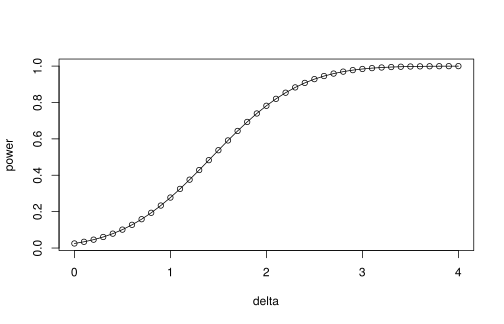
\includegraphics{twolevelconf_files/figure-latex/unnamed-chunk-17-1.pdf}

\hypertarget{uxcd5cuxc885-uxbaa8uxd615}{%
\section{최종 모형}\label{uxcd5cuxc885-uxbaa8uxd615}}

위의 핵심요인의 선별 결과를 고려하여 주요인 \(A\), \(B\), \(C\), \(D\) 와 상호작용 효과 \(AC\) 와 \(AD\) 를 포함하는
축소된 모형을 최종모형으로 적합해 보자. 축소모형에는 당연히 블럭효과도 포함해야 한다. 또한 오차항에는 블럭과 교럭돤 상호작용 효과들과
축소모형에 포함된 효과들을 제외한 다른 효과들이 풀링된다.

\[ SS_E = SS_{B \times C} + SS_{B \times D} + SS_{C \times D} + SS_{A \times B \times C} + SS_{A \times B \times D } + SS_{A \times B \times C \times D}\]

\begin{Shaded}
\begin{Highlighting}[]
\NormalTok{finalmodel }\OtherTok{\textless{}{-}} \FunctionTok{lm}\NormalTok{(y }\SpecialCharTok{\textasciitilde{}}\NormalTok{ block }\SpecialCharTok{+}\NormalTok{ A }\SpecialCharTok{+}\NormalTok{B }\SpecialCharTok{+}\NormalTok{ C}\SpecialCharTok{+}\NormalTok{ D }\SpecialCharTok{+}\NormalTok{ A}\SpecialCharTok{:}\NormalTok{C }\SpecialCharTok{+}\NormalTok{ A}\SpecialCharTok{:}\NormalTok{D, }\AttributeTok{data=}\NormalTok{df)}
\FunctionTok{anova}\NormalTok{(finalmodel)}
\end{Highlighting}
\end{Shaded}

\begin{verbatim}
## Analysis of Variance Table
## 
## Response: y
##           Df   Sum Sq  Mean Sq  F value     Pr(>F)    
## block      3   38.187   12.729  0.64793 0.61234985    
## A          1 1870.562 1870.562 95.21421 6.6601e-05 ***
## B          1   39.062   39.062  1.98834 0.20818928    
## C          1  390.063  390.063 19.85472 0.00430203 ** 
## D          1  855.563  855.563 43.54931 0.00058207 ***
## A:C        1 1314.062 1314.062 66.88759 0.00017998 ***
## A:D        1 1105.562 1105.562 56.27466 0.00029022 ***
## Residuals  6  117.875   19.646                        
## ---
## Signif. codes:  0 '***' 0.001 '**' 0.01 '*' 0.05 '.' 0.1 ' ' 1
\end{verbatim}

\hypertarget{uxc0c1uxd638uxc791uxc6a9-uxadf8uxb9bc}{%
\section{상호작용 그림}\label{uxc0c1uxd638uxc791uxc6a9-uxadf8uxb9bc}}

\begin{Shaded}
\begin{Highlighting}[]
\FunctionTok{with}\NormalTok{(df, }\FunctionTok{interaction.plot}\NormalTok{(}\AttributeTok{x.factor =}\NormalTok{ A, }\AttributeTok{trace.factor =}\NormalTok{ C,  }\AttributeTok{response =}\NormalTok{ y))}
\end{Highlighting}
\end{Shaded}

\includegraphics{twolevelconf_files/figure-latex/unnamed-chunk-19-1.pdf}

\begin{Shaded}
\begin{Highlighting}[]
\FunctionTok{with}\NormalTok{(df, }\FunctionTok{interaction.plot}\NormalTok{(}\AttributeTok{x.factor =}\NormalTok{ A, }\AttributeTok{trace.factor =}\NormalTok{ D,  }\AttributeTok{response =}\NormalTok{ y))}
\end{Highlighting}
\end{Shaded}

\includegraphics{twolevelconf_files/figure-latex/unnamed-chunk-20-1.pdf}

\hypertarget{exerxise8}{%
\chapter{8장 연습문제}\label{exerxise8}}

다음은 8장의 연습문제를 풀 때 도음이 되는 R 프로그램이다.

\hypertarget{uxc5f0uxc2b5uxbb38uxc81c-1}{%
\section{연습문제 1}\label{uxc5f0uxc2b5uxbb38uxc81c-1}}

\begin{Shaded}
\begin{Highlighting}[]
\NormalTok{X1 }\OtherTok{\textless{}{-}} \FunctionTok{FrF2}\NormalTok{(}\AttributeTok{nruns=}\DecValTok{16}\NormalTok{, }\AttributeTok{nfactors=}\DecValTok{4}\NormalTok{, }\AttributeTok{randomize =} \ConstantTok{FALSE}\NormalTok{,  }\AttributeTok{default.level=}\FunctionTok{c}\NormalTok{(}\DecValTok{0}\NormalTok{,}\DecValTok{1}\NormalTok{))}
\end{Highlighting}
\end{Shaded}

\begin{verbatim}
## creating full factorial with 16 runs ...
\end{verbatim}

\begin{Shaded}
\begin{Highlighting}[]
\NormalTok{X1}
\end{Highlighting}
\end{Shaded}

\begin{verbatim}
##    A B C D
## 1  0 0 0 0
## 2  1 0 0 0
## 3  0 1 0 0
## 4  1 1 0 0
## 5  0 0 1 0
## 6  1 0 1 0
## 7  0 1 1 0
## 8  1 1 1 0
## 9  0 0 0 1
## 10 1 0 0 1
## 11 0 1 0 1
## 12 1 1 0 1
## 13 0 0 1 1
## 14 1 0 1 1
## 15 0 1 1 1
## 16 1 1 1 1
## class=design, type= full factorial
\end{verbatim}

\begin{Shaded}
\begin{Highlighting}[]
\FunctionTok{yates}\NormalTok{(}\FunctionTok{rep}\NormalTok{(}\DecValTok{0}\NormalTok{,}\DecValTok{16}\NormalTok{))}
\end{Highlighting}
\end{Shaded}

\begin{verbatim}
##    A    B   AB    C   AC   BC  ABC    D   AD   BD  ABD   CD  ACD  BCD ABCD 
##    0    0    0    0    0    0    0    0    0    0    0    0    0    0    0 
## attr(,"mean")
##   
## 0
\end{verbatim}

\begin{Shaded}
\begin{Highlighting}[]
\NormalTok{Def.contrast1 }\OtherTok{\textless{}{-}} \FunctionTok{c}\NormalTok{(}\DecValTok{1}\NormalTok{,}\DecValTok{1}\NormalTok{,}\DecValTok{1}\NormalTok{,}\DecValTok{1}\NormalTok{)}
\FunctionTok{conf.design}\NormalTok{(}\AttributeTok{G=}\NormalTok{Def.contrast1 , }\AttributeTok{p=}\DecValTok{2}\NormalTok{, }\AttributeTok{block.name =} \StringTok{"블럭"}\NormalTok{, }\AttributeTok{treatment.names=}\FunctionTok{c}\NormalTok{(}\StringTok{"A"}\NormalTok{, }\StringTok{"B"}\NormalTok{, }\StringTok{"C"}\NormalTok{, }\StringTok{"D"}\NormalTok{))}
\end{Highlighting}
\end{Shaded}

\begin{verbatim}
##    블럭 A B C D
## 1     0 0 0 0 0
## 2     0 1 1 0 0
## 3     0 1 0 1 0
## 4     0 0 1 1 0
## 5     0 1 0 0 1
## 6     0 0 1 0 1
## 7     0 0 0 1 1
## 8     0 1 1 1 1
## 9     1 1 0 0 0
## 10    1 0 1 0 0
## 11    1 0 0 1 0
## 12    1 1 1 1 0
## 13    1 0 0 0 1
## 14    1 1 1 0 1
## 15    1 1 0 1 1
## 16    1 0 1 1 1
\end{verbatim}

\hypertarget{uxc5f0uxc2b5uxbb38uxc81c-4}{%
\section{연습문제 4}\label{uxc5f0uxc2b5uxbb38uxc81c-4}}

\begin{Shaded}
\begin{Highlighting}[]
\NormalTok{X2 }\OtherTok{\textless{}{-}} \FunctionTok{FrF2}\NormalTok{(}\AttributeTok{nruns=}\DecValTok{8}\NormalTok{, }\AttributeTok{nfactors=}\DecValTok{3}\NormalTok{, }\AttributeTok{randomize =} \ConstantTok{FALSE}\NormalTok{,  }\AttributeTok{default.level=}\FunctionTok{c}\NormalTok{(}\DecValTok{0}\NormalTok{,}\DecValTok{1}\NormalTok{))}
\end{Highlighting}
\end{Shaded}

\begin{verbatim}
## creating full factorial with 8 runs ...
\end{verbatim}

\begin{Shaded}
\begin{Highlighting}[]
\NormalTok{X2}
\end{Highlighting}
\end{Shaded}

\begin{verbatim}
##   A B C
## 1 0 0 0
## 2 1 0 0
## 3 0 1 0
## 4 1 1 0
## 5 0 0 1
## 6 1 0 1
## 7 0 1 1
## 8 1 1 1
## class=design, type= full factorial
\end{verbatim}

\begin{Shaded}
\begin{Highlighting}[]
\FunctionTok{yates}\NormalTok{(}\FunctionTok{rep}\NormalTok{(}\DecValTok{0}\NormalTok{,}\DecValTok{8}\NormalTok{))}
\end{Highlighting}
\end{Shaded}

\begin{verbatim}
##   A   B  AB   C  AC  BC ABC 
##   0   0   0   0   0   0   0 
## attr(,"mean")
##   
## 0
\end{verbatim}

\begin{Shaded}
\begin{Highlighting}[]
\NormalTok{Def.contrast2 }\OtherTok{\textless{}{-}} \FunctionTok{c}\NormalTok{(}\DecValTok{1}\NormalTok{,}\DecValTok{1}\NormalTok{,}\DecValTok{1}\NormalTok{)}
\FunctionTok{conf.design}\NormalTok{(}\AttributeTok{G=}\NormalTok{Def.contrast2 , }\AttributeTok{p=}\DecValTok{2}\NormalTok{, }\AttributeTok{block.name =} \StringTok{"블럭"}\NormalTok{, }\AttributeTok{treatment.names=}\FunctionTok{c}\NormalTok{(}\StringTok{"A"}\NormalTok{, }\StringTok{"B"}\NormalTok{, }\StringTok{"C"}\NormalTok{))}
\end{Highlighting}
\end{Shaded}

\begin{verbatim}
##   블럭 A B C
## 1    0 0 0 0
## 2    0 1 1 0
## 3    0 1 0 1
## 4    0 0 1 1
## 5    1 1 0 0
## 6    1 0 1 0
## 7    1 0 0 1
## 8    1 1 1 1
\end{verbatim}

\hypertarget{uxc5f0uxc2b5uxbb38uxc81c-10}{%
\section{연습문제 10}\label{uxc5f0uxc2b5uxbb38uxc81c-10}}

\begin{Shaded}
\begin{Highlighting}[]
\NormalTok{X3 }\OtherTok{\textless{}{-}} \FunctionTok{FrF2}\NormalTok{(}\AttributeTok{nruns=}\DecValTok{64}\NormalTok{, }\AttributeTok{nfactors=}\DecValTok{6}\NormalTok{, }\AttributeTok{randomize =} \ConstantTok{FALSE}\NormalTok{,  }\AttributeTok{default.level=}\FunctionTok{c}\NormalTok{(}\DecValTok{0}\NormalTok{,}\DecValTok{1}\NormalTok{))}
\end{Highlighting}
\end{Shaded}

\begin{verbatim}
## creating full factorial with 64 runs ...
\end{verbatim}

\begin{Shaded}
\begin{Highlighting}[]
\NormalTok{X3}
\end{Highlighting}
\end{Shaded}

\begin{verbatim}
##    A B C D E F
## 1  0 0 0 0 0 0
## 2  1 0 0 0 0 0
## 3  0 1 0 0 0 0
## 4  1 1 0 0 0 0
## 5  0 0 1 0 0 0
## 6  1 0 1 0 0 0
## 7  0 1 1 0 0 0
## 8  1 1 1 0 0 0
## 9  0 0 0 1 0 0
## 10 1 0 0 1 0 0
## 11 0 1 0 1 0 0
## 12 1 1 0 1 0 0
## 13 0 0 1 1 0 0
## 14 1 0 1 1 0 0
## 15 0 1 1 1 0 0
## 16 1 1 1 1 0 0
## 17 0 0 0 0 1 0
## 18 1 0 0 0 1 0
## 19 0 1 0 0 1 0
## 20 1 1 0 0 1 0
## 21 0 0 1 0 1 0
## 22 1 0 1 0 1 0
## 23 0 1 1 0 1 0
## 24 1 1 1 0 1 0
## 25 0 0 0 1 1 0
## 26 1 0 0 1 1 0
## 27 0 1 0 1 1 0
## 28 1 1 0 1 1 0
## 29 0 0 1 1 1 0
## 30 1 0 1 1 1 0
## 31 0 1 1 1 1 0
## 32 1 1 1 1 1 0
## 33 0 0 0 0 0 1
## 34 1 0 0 0 0 1
## 35 0 1 0 0 0 1
## 36 1 1 0 0 0 1
## 37 0 0 1 0 0 1
## 38 1 0 1 0 0 1
## 39 0 1 1 0 0 1
## 40 1 1 1 0 0 1
## 41 0 0 0 1 0 1
## 42 1 0 0 1 0 1
## 43 0 1 0 1 0 1
## 44 1 1 0 1 0 1
## 45 0 0 1 1 0 1
## 46 1 0 1 1 0 1
## 47 0 1 1 1 0 1
## 48 1 1 1 1 0 1
## 49 0 0 0 0 1 1
## 50 1 0 0 0 1 1
## 51 0 1 0 0 1 1
## 52 1 1 0 0 1 1
## 53 0 0 1 0 1 1
## 54 1 0 1 0 1 1
## 55 0 1 1 0 1 1
## 56 1 1 1 0 1 1
## 57 0 0 0 1 1 1
## 58 1 0 0 1 1 1
## 59 0 1 0 1 1 1
## 60 1 1 0 1 1 1
## 61 0 0 1 1 1 1
## 62 1 0 1 1 1 1
## 63 0 1 1 1 1 1
## 64 1 1 1 1 1 1
## class=design, type= full factorial
\end{verbatim}

\begin{Shaded}
\begin{Highlighting}[]
\FunctionTok{yates}\NormalTok{(}\FunctionTok{rep}\NormalTok{(}\DecValTok{0}\NormalTok{,}\DecValTok{64}\NormalTok{))}
\end{Highlighting}
\end{Shaded}

\begin{verbatim}
##      A      B     AB      C     AC     BC    ABC      D     AD     BD    ABD 
##      0      0      0      0      0      0      0      0      0      0      0 
##     CD    ACD    BCD   ABCD      E     AE     BE    ABE     CE    ACE    BCE 
##      0      0      0      0      0      0      0      0      0      0      0 
##   ABCE     DE    ADE    BDE   ABDE    CDE   ACDE   BCDE  ABCDE      F     AF 
##      0      0      0      0      0      0      0      0      0      0      0 
##     BF    ABF     CF    ACF    BCF   ABCF     DF    ADF    BDF   ABDF    CDF 
##      0      0      0      0      0      0      0      0      0      0      0 
##   ACDF   BCDF  ABCDF     EF    AEF    BEF   ABEF    CEF   ACEF   BCEF  ABCEF 
##      0      0      0      0      0      0      0      0      0      0      0 
##    DEF   ADEF   BDEF  ABDEF   CDEF  ACDEF  BCDEF ABCDEF 
##      0      0      0      0      0      0      0      0 
## attr(,"mean")
##   
## 0
\end{verbatim}

\begin{Shaded}
\begin{Highlighting}[]
\NormalTok{Def.contrast3 }\OtherTok{\textless{}{-}}   \FunctionTok{matrix}\NormalTok{(}\FunctionTok{c}\NormalTok{(}\DecValTok{1}\NormalTok{,}\DecValTok{1}\NormalTok{,}\DecValTok{1}\NormalTok{,}\DecValTok{1}\NormalTok{,}\DecValTok{0}\NormalTok{,}\DecValTok{0}\NormalTok{, }\DecValTok{1}\NormalTok{,}\DecValTok{1}\NormalTok{,}\DecValTok{0}\NormalTok{,}\DecValTok{0}\NormalTok{,}\DecValTok{1}\NormalTok{,}\DecValTok{1}\NormalTok{), }\DecValTok{2}\NormalTok{,}\DecValTok{6}\NormalTok{, }\AttributeTok{byrow=}\ConstantTok{TRUE}\NormalTok{)}
\FunctionTok{conf.design}\NormalTok{(}\AttributeTok{G=}\NormalTok{Def.contrast3 , }\AttributeTok{p=}\DecValTok{2}\NormalTok{, }\AttributeTok{block.name =} \StringTok{"블럭"}\NormalTok{, }\AttributeTok{treatment.names=}\FunctionTok{c}\NormalTok{(}\StringTok{"A"}\NormalTok{, }\StringTok{"B"}\NormalTok{, }\StringTok{"C"}\NormalTok{, }\StringTok{"D"}\NormalTok{, }\StringTok{"E"}\NormalTok{, }\StringTok{"F"}\NormalTok{))}
\end{Highlighting}
\end{Shaded}

\begin{verbatim}
##    블럭 A B C D E F
## 1    00 0 0 0 0 0 0
## 2    00 1 1 0 0 0 0
## 3    00 0 0 1 1 0 0
## 4    00 1 1 1 1 0 0
## 5    00 1 0 1 0 1 0
## 6    00 0 1 1 0 1 0
## 7    00 1 0 0 1 1 0
## 8    00 0 1 0 1 1 0
## 9    00 1 0 1 0 0 1
## 10   00 0 1 1 0 0 1
## 11   00 1 0 0 1 0 1
## 12   00 0 1 0 1 0 1
## 13   00 0 0 0 0 1 1
## 14   00 1 1 0 0 1 1
## 15   00 0 0 1 1 1 1
## 16   00 1 1 1 1 1 1
## 17   01 1 0 1 0 0 0
## 18   01 0 1 1 0 0 0
## 19   01 1 0 0 1 0 0
## 20   01 0 1 0 1 0 0
## 21   01 0 0 0 0 1 0
## 22   01 1 1 0 0 1 0
## 23   01 0 0 1 1 1 0
## 24   01 1 1 1 1 1 0
## 25   01 0 0 0 0 0 1
## 26   01 1 1 0 0 0 1
## 27   01 0 0 1 1 0 1
## 28   01 1 1 1 1 0 1
## 29   01 1 0 1 0 1 1
## 30   01 0 1 1 0 1 1
## 31   01 1 0 0 1 1 1
## 32   01 0 1 0 1 1 1
## 33   10 0 0 1 0 0 0
## 34   10 1 1 1 0 0 0
## 35   10 0 0 0 1 0 0
## 36   10 1 1 0 1 0 0
## 37   10 1 0 0 0 1 0
## 38   10 0 1 0 0 1 0
## 39   10 1 0 1 1 1 0
## 40   10 0 1 1 1 1 0
## 41   10 1 0 0 0 0 1
## 42   10 0 1 0 0 0 1
## 43   10 1 0 1 1 0 1
## 44   10 0 1 1 1 0 1
## 45   10 0 0 1 0 1 1
## 46   10 1 1 1 0 1 1
## 47   10 0 0 0 1 1 1
## 48   10 1 1 0 1 1 1
## 49   11 1 0 0 0 0 0
## 50   11 0 1 0 0 0 0
## 51   11 1 0 1 1 0 0
## 52   11 0 1 1 1 0 0
## 53   11 0 0 1 0 1 0
## 54   11 1 1 1 0 1 0
## 55   11 0 0 0 1 1 0
## 56   11 1 1 0 1 1 0
## 57   11 0 0 1 0 0 1
## 58   11 1 1 1 0 0 1
## 59   11 0 0 0 1 0 1
## 60   11 1 1 0 1 0 1
## 61   11 1 0 0 0 1 1
## 62   11 0 1 0 0 1 1
## 63   11 1 0 1 1 1 1
## 64   11 0 1 1 1 1 1
\end{verbatim}

  \bibliography{book.bib,packages.bib}

\end{document}
